%!TEX root = ../report.tex
\documentclass[../report.tex]{subfiles}
\begin{document}
    \chapter{Implementation}
    This chapter describes gives implementation details of the experiments conducted during this thesis work. In the beginning architectural specifications of GestaltMatcher are provided. Subsequently, we describe the procedure to integrate explanation methods with the model. Furthermore, implementation details of the experiments proposed in the previous chapter are discussed. Finally, the evaluation questionnaire is presented.
    \section{GestaltMatcher Architecture}
    The procedure to diagnose rare-genetic syndromes from patient faces using GestaltMatcher is described in a detailed manner in Chapter 2 \ref{}. This section describes the architecture of its underlying Convolutional Neural Network (CNN) backbone and steps involved in preprocessing its input images. The pipeline shown in Figure \ref{fig_gm_pipeline} illustrates the sequence of steps involved in processing a patient photo using GestaltMatcher.
    \begin{figure}[ht]
    	\hspace*{-0.5cm}      
    	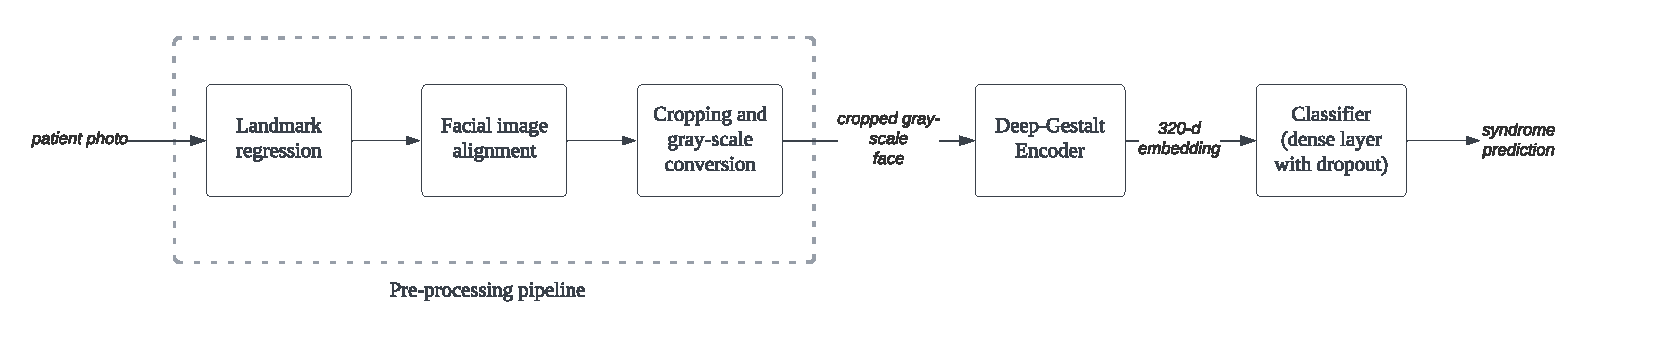
\includegraphics[scale=0.62]{chapter4/gestalt_matcher_pipeline.pdf}
    	\caption{Illustration of the pipleline to process a patient photo using GestaltMatcher}
    	\label{fig_gm_pipeline}
    \end{figure}
	
	\subsubsection{Pre-processing Pipeline}
	The pre-processing pipeline is responsible for detecting facial landmarks and aligning the orientation of a given patient photo, and finally cropping the face from it. Authors of GestaltMatcher use RetinaFace \cite{deng2020retinaface} to fetch detect landmark points from a patient's facial image.  In a nutshell, RetinaFace is a single-stage, multi-scale face localization method which employs multi-task learning to perform five different tasks: face detection, landmark position and score regression,  3D position and pixel correspondence prediction. It uses a Resnet-50 \cite{he2016deep} backbone. The facial landmark coordinates outputted by RetinaFace is used to crop and align faces from patient photos. The facial images are resized to 100 x 100, and converted to gray-scale before feeding them to the GestaltMatcher neural network model.

	\subsubsection{Architecture Specifications}
	GestaltMatcher consists of an encoder and a classifier module. The encoder is called as "Deep Gestalt encoder", named after the work \cite{Gurovich2019} in which its architecture was first proposed. Deep Gestalt encoder uses a CNN to extract discriminative features from input facial images, and represent them in 320-dimensional embedding space called the \enquote{Clinical Face Phenotype Space} (CFPS). As explained in Chapter 2\ref{}, an embedding  projected onto the CFPS can be used to match its corresponding patient photo to a gallery of facial portraits of unsolved or solved cases. For syndrome recognition, a fully-connected layer, which acts as classifier, is appended to the encoder. 
	\begin{figure}[ht]
	\hspace*{1.0cm}      
	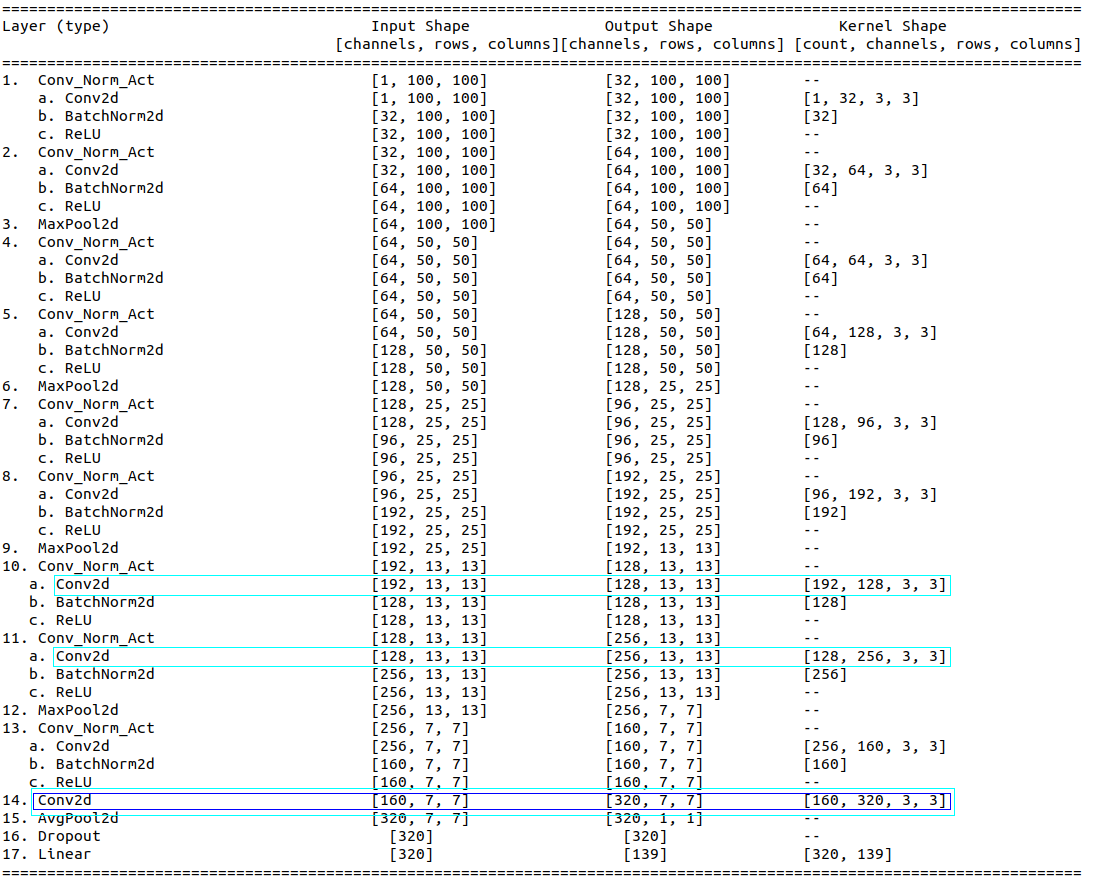
\includegraphics[scale=0.4]{chapter5/gestalt_matcher_arch.png}
	\caption{Architecture of the CNN in GestaltMatcher. The convolution layer 14 used to generate attribution maps using GradCAM and HiResCAM methods
	is highlighted using a blue box. Layers (10.a, 11.a and 14) that are used by the CustomGradCAM method are highlighted using cyan boxes. }
	\label{fig_arch_gest_matcher}
	\end{figure}

	\subsubsection{Model Training}
	The presented neural network is first trained on facial images from the CASIA-WebFace \cite{yi2014learning} dataset. Subsequently, it is trained on 139 frequent-syndrome classes listed in the GestaltMatcher paper \cite{hsieh2022gestaltmatcher}. The training details are presented in \ref{}. <Accuracy>
    \section{Explanation Methods - GestaltMatcher Integration}
     \begin{figure}[H]
    	\hspace*{0.5cm}      
    	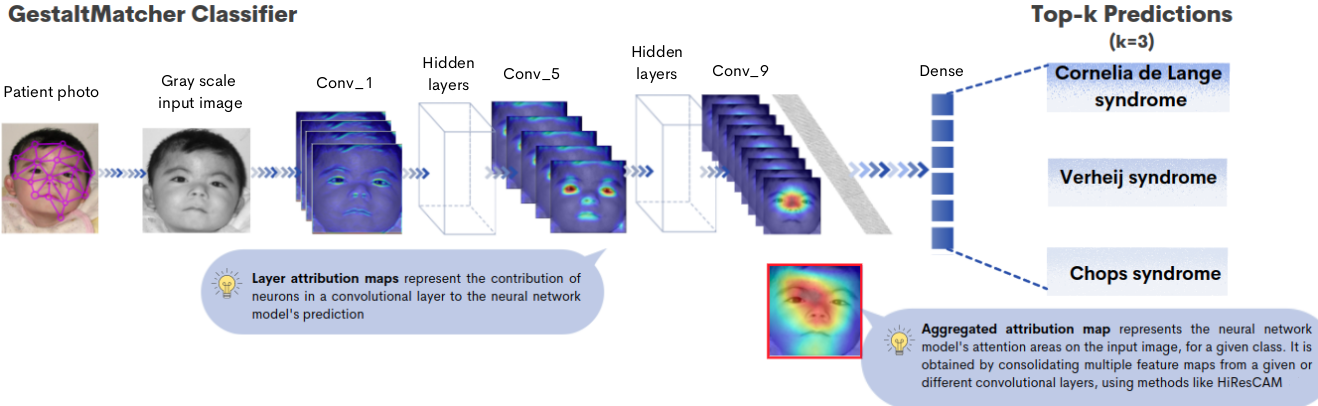
\includegraphics[scale=0.45]{chapter5/xai_gestalt_matcher_intergration.png}
    	\caption{An illustration of attribution map computation from the GestaltMatcher model}
    	\label{fig_gm_pipeline}
    \end{figure}
	The Class Activation Mapping (CAM) methods used for this work typically generate class-specific attribution maps, by evaluating contributions of neurons in a given convolutional layer to the model output. Therefore, the choice of target convolutional layer plays a vital role. Selvaraju \etal \cite{selvaraju2017grad} recommend to use the last convolutional layers, as they contain more high-level semantic and spatial information, when compared to earlier layers, which have smaller receptive fields. The same is reinforced by Muhammad \etal \cite{muhammad2020eigen}. We validated this recommendation by computing and comparing attribution maps generated from all ten convolutional layers, using both GradCAM and HiResCAM techniques. FullGrad was excluded from this analysis, as the method is layer-agnostic in nature.
	\begin{sidewaysfigure}
		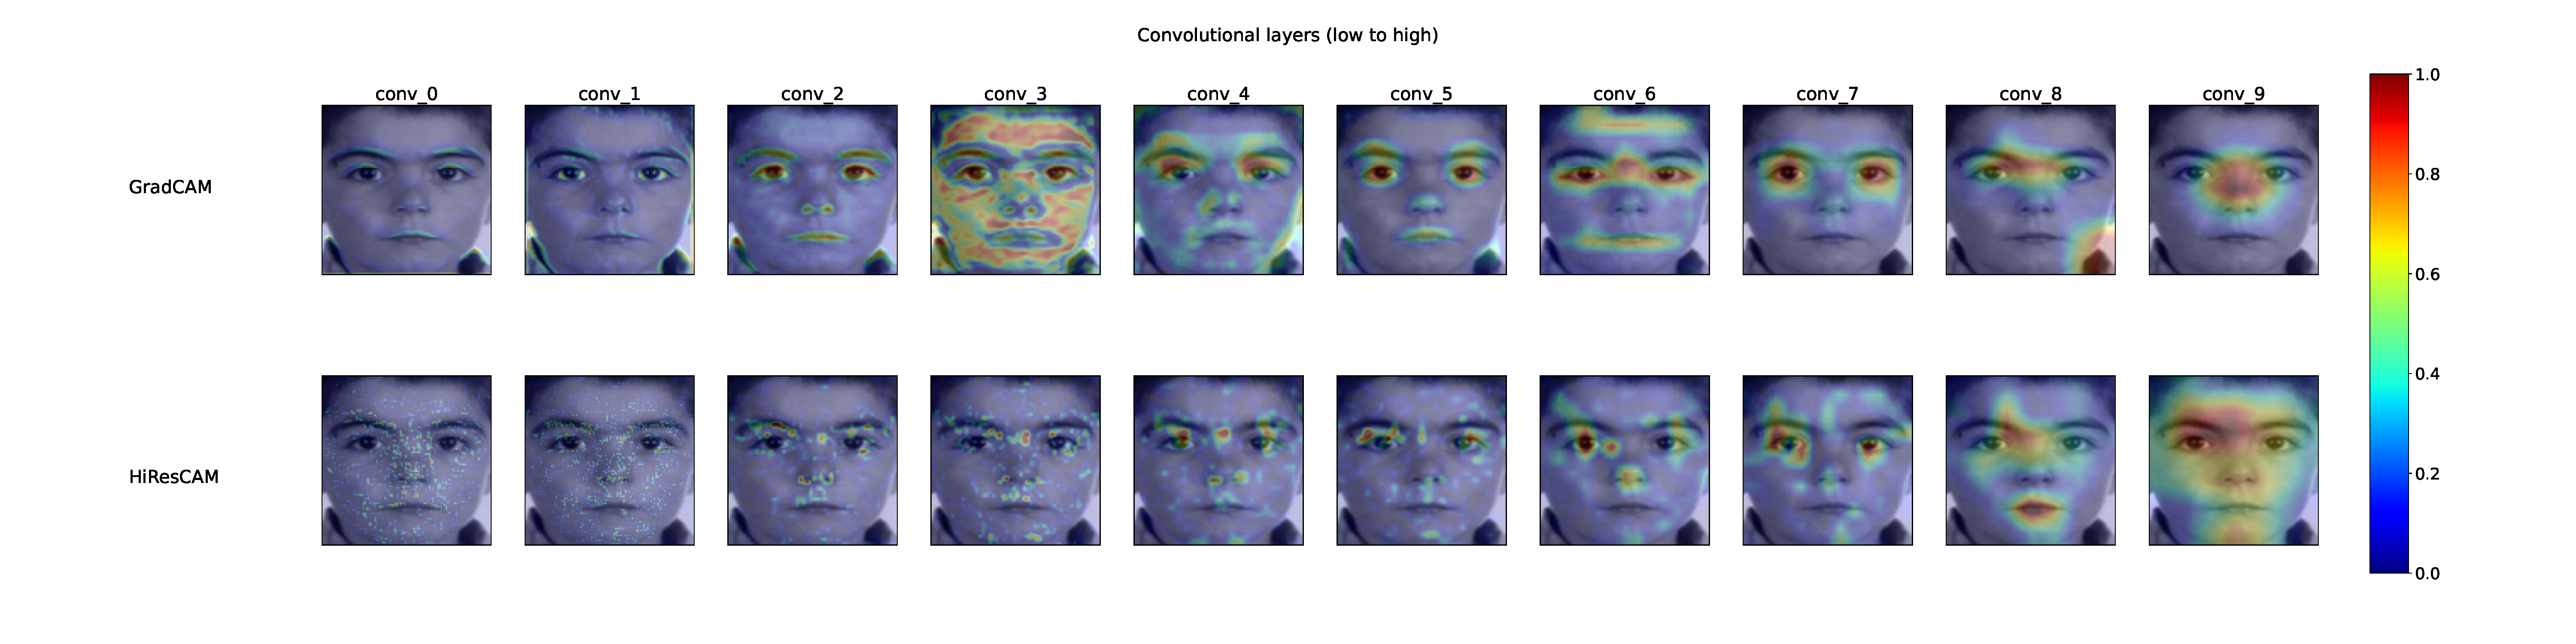
\includegraphics[scale=0.22, trim = 1cm 2.50cm 1cm 2.50cm, clip]{chapter5/layer_attribution1_synd1.pdf}
	   
		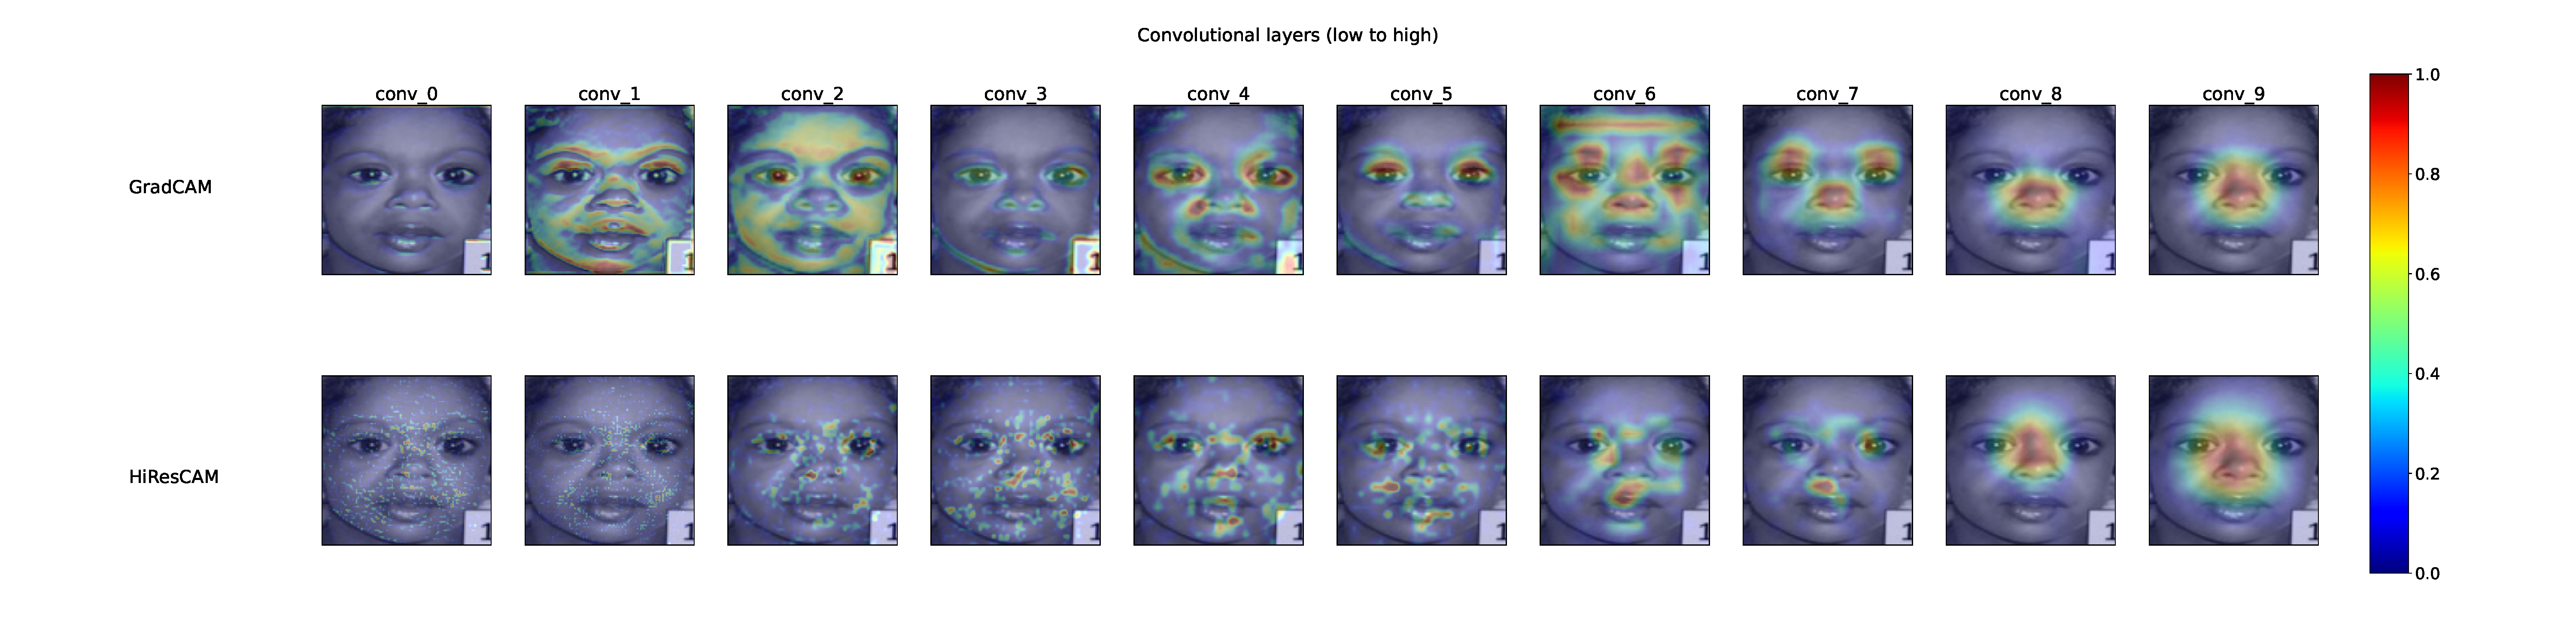
\includegraphics[scale=0.22, trim = 1cm 2.50cm 1cm 2.50cm, clip]{chapter5/layer_attribution3_synd1.pdf}
		\label{fig_gm_pipeline}	      
		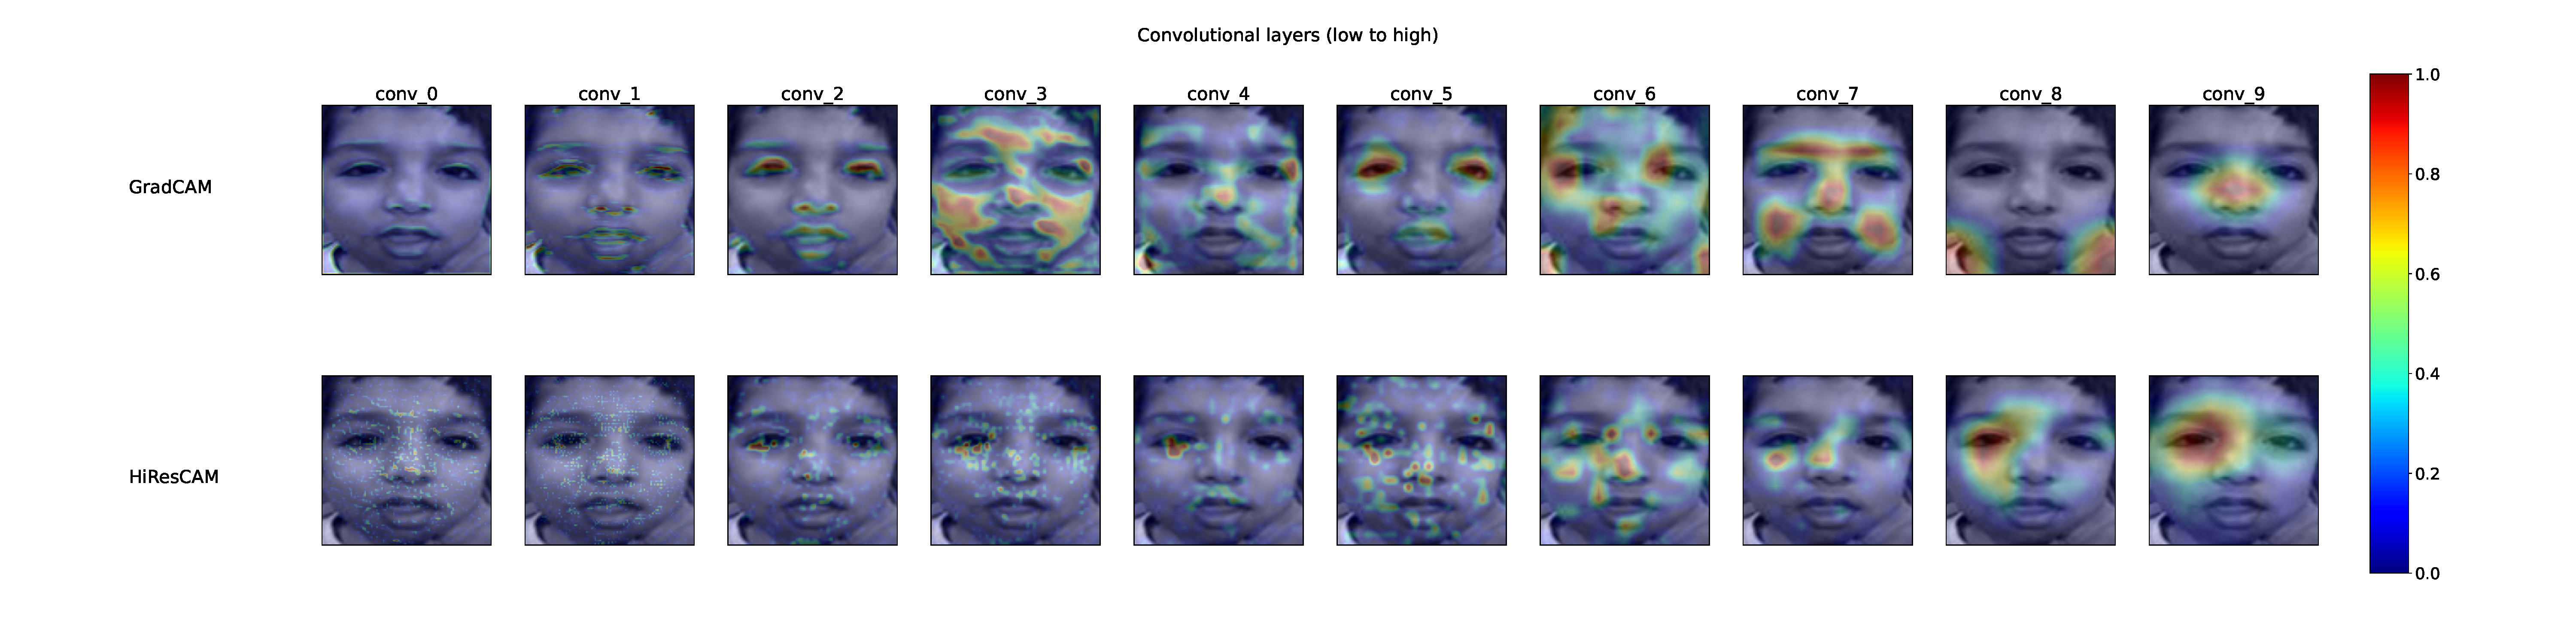
\includegraphics[scale=0.22, trim = 1cm 2.50cm 1cm 2.50cm, clip]{chapter5/layer_attribution_synd2.pdf}
		\caption{Layer-wise visualization of attribution maps generated by GradCAM and HiResCAM methods.}
		\label{fig_layer_visual}
	\end{sidewaysfigure}
	Based on the recommendation and our observations, we chose layer 14 (refer conv\_9 in Figure \ref{fig_layer_visual}), the last convolutional layer to compute attribution maps.\\
	\subsubsection{CustomGradCAM}
	Apart from the last convolution layer, we also observed that applying GradCAM to layers 10.a and 11.a produced visualizations in which certain key features of human face are highlighted (refer conv\_6 and conv\_7 in Figure \ref{fig_layer_visual}). Therefore, in order to include the layers in our scope, we averaged their attribution maps along with the ones produced by layer 14. The resulting map is presented under the name of \enquote{CustomGradCAM}. We used the Application Programming Interfaces (APIs) offered by PyTorch \cite{paszke2019pytorch}, Captum \cite{kokhlikyan2020captum} and an open-source library \cite{jacobgilpytorchcam} to integrate the explanation methods to the GestaltMatcher classifier model.
	\subsection{Visualization Details}
	 Captum's visualizer tool was used to generate color coded attribution maps. We post-processed attribution maps to remove noise and visual artifacts. This section provides details on visualization parameters and the post-processing procedure.
	\subsubsection{Interpolation}
	The attribution maps generated by layer-specific methods such as GradCAM and HiResCAM are shaped identical to the feature maps outputted by the target layers. For example, layer 14 of the gestaltmatcher model spits out 320 7x7 (height x width) feature maps, and any attribution map generated from the layer is of dimensions 7x7 (height x width). The bilinear interpolation technique \cite{bovik2009essential} was used to rescale attribution maps to the input image size of 100x100 (height x width), so that the map could be overlaid on the input image.
	\subsubsection{Attribution Sign and Representation}
	We considered only positive attribution values for visualization and used the \enquote{jet} colormap scheme offered by Captum's \cite{kokhlikyan2020captum} visualization tool.
	\subsubsection{Smoothing Attribution Maps}
	Test Time Augmentation (TTA) is a commonly used technique to boost the performance of image classification models \cite{simonyan2014very}. During the inference process for a given input image, instead of passing the actual sample, its augmented counterparts are fed to obtain predictions from the model. Thus obtained predictions are averaged to obtain the final output. Augmented copies are obtained by applying transformations such as rotations and flips to the original input image.\\
	In our work, we used TTA to enhance the quality of generated attribution maps. Augmented copies of every test input image were obtained by individually applying horizontal flipping and multiplications (with factors of 0.9, 1 and 1.1) operations. Attribution maps were generated for each augmented copy, and finally averaged to obtain the smoothened map. Attribution maps produced from HiResCAM were exempted from TTA based on the guidelines provided by Jacob Gildendblat \cite{jacobgilpytorchcam}.
	
    \section{Experiments}
    Implementation details of the conducted set of experiments are presented in this section.
    \subsection{Patient-wise Attribution Map Generation}
    Patient-wise attribution maps are generated by applying the chosen set of methods to individual patient images. The attributions are computed with respect to the logit scores of the samples' ground truth classes. This is because the attribution \enquote{methods work only when the classification result is correct} \cite{muhammad2020eigen}. However, an experiment was also conducted to observe the differences between explanations of misclassified samples, obtained by computing attributions with respect to their ground truth and predicted labels. Its results are discussed in the next chapter.
    \begin{figure}[H]
    	\hspace*{0cm}      
    	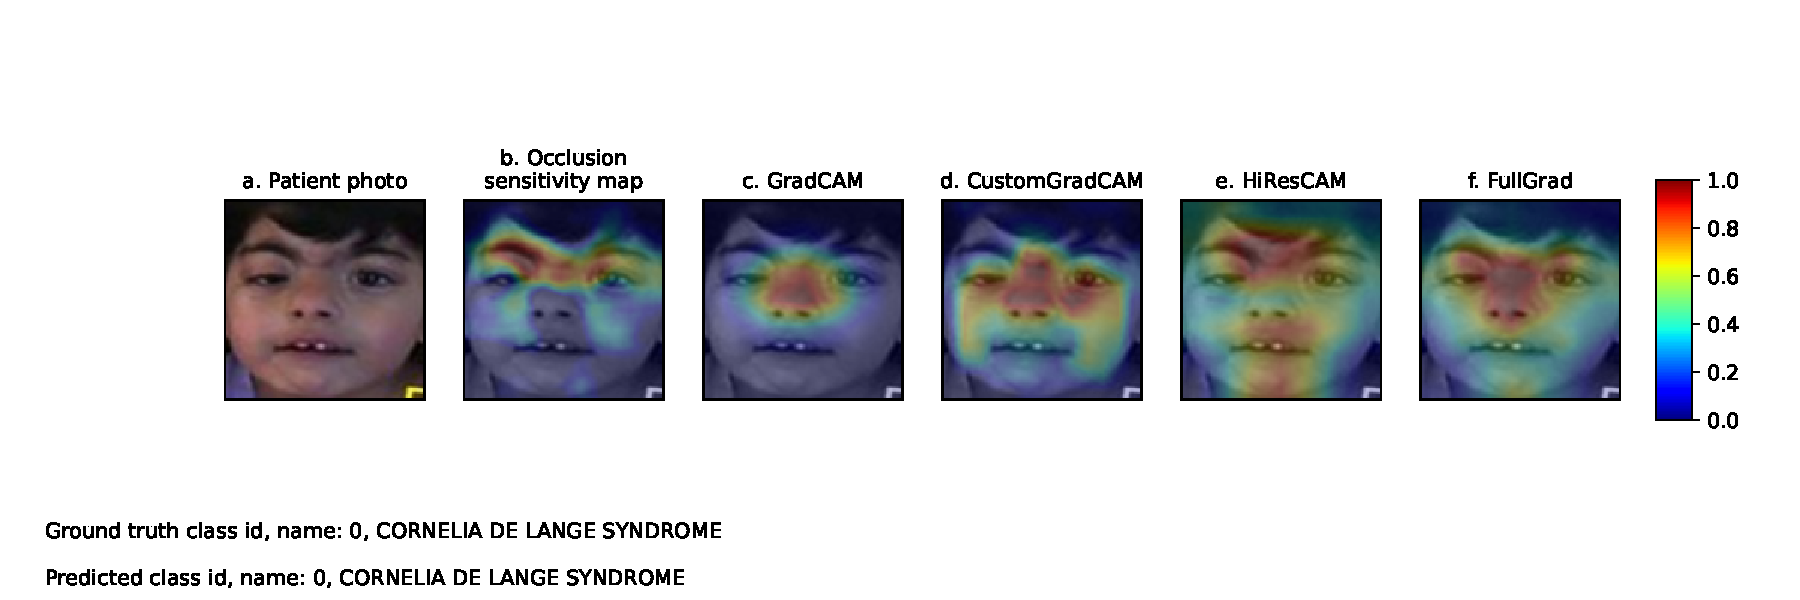
\includegraphics[scale=0.55,trim = 1cm 2.50cm 1cm 2.50cm, clip]{chapter5/example_attribution.pdf}
    	\caption{An example for patient-wise attribution maps}
    	\label{fig_gm_pipeline}
    \end{figure}
    \subsection{Composite Face Generation}
    Composite faces are generated with an intent to synthesize a characteristic face for each genetic syndrome class under our scope. Concisely put, they are obtained from aligning and averaging facial images of each category separately. This section provides a detailed description of the process involved.
       \begin{figure}[H]
    	\hspace*{-0.5cm}      
    	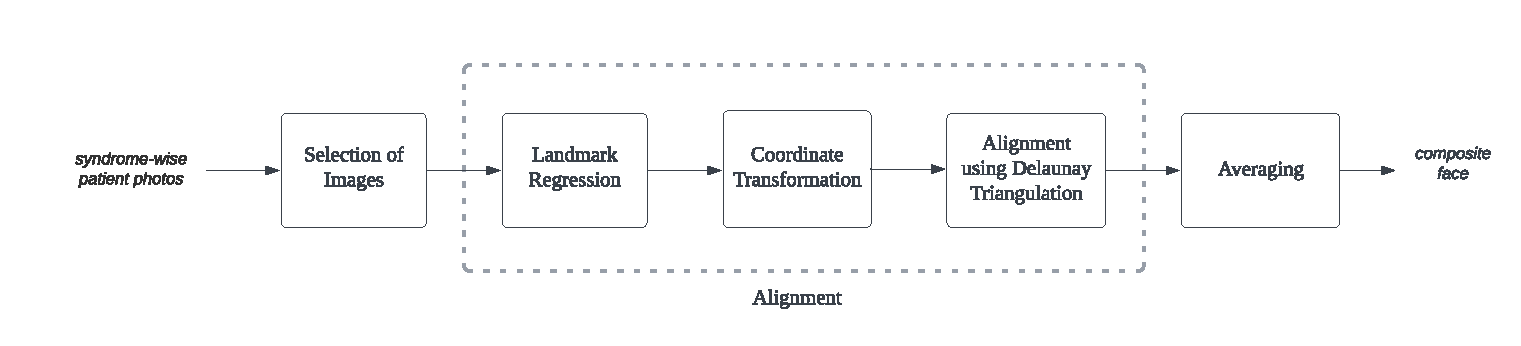
\includegraphics[scale=0.66]{chapter5/composite_face_pipeline.pdf}
    	\caption{Block diagram representing composite face generation process}
    	\label{fig_gm_pipeline}
    \end{figure}
    
    \subsubsection{a. Selection of Images}
    The first step involved in generating composite faces is to select the right consituent images. A considerable number of images in \ref{} GMDB are characterized by poor visual quality and/or presence of artifacts. A few such as the ones shown in Figure \ref{} also contain objects like nasal catheter tubes, spectacles, and black strips which were introduced to conceal patient identities. Therefore, we hand picked images from each of 139 syndrome classes to remove the unsuitable candidates for generating composite faces.
    
    <Bad image examples>
    \subsubsection{b. Facial Landmark Regression}
    Landmark points act as anchors to align the constituent images of composite faces. 68 landmark points are calculated for each input facial image using the dlib \footnote{dlib library - \url{http://dlib.net/}.}library's face detector functionality. Internally, dlib uses a CNN based max-margin object detector to perform the task.
    <Facial landmark example image>
    <dlib link>
    \subsubsection{c. Coordinate Transformation}
    The next step warps the consituent facial images in a such a way that their landmark points corresponding to the right corner of the right eye and the left corner of the left eye are shifted to locations $P_{1}$ (0.3 x image width, 0.3 x image height) and $P_{2}$ (0.7 x image width, 0.3 x image height) respectively. In practice this is achieved by computing and applying a similarity transformation matrix using OpenCV library's \enquote{estimateRigidTransform} method.
    
    Similarity transformation \cite{hartley2003multiple} is a specialization of projective transformations, composed of an euclidean transformation (rotation and translation), and an isotropic scaling. Planar similarity transformation has four Degrees Of Freedom (DOFs) can be expressed in the following form:
    <equation>
    
    Planar affine transformation has two more DOFs offered by non-isotropic scaling and shear. A planar affine transformation can represented in the form of following matrix:
    
    \subsubsection{d. Facial Alignment using Delaunay Triangulation}
    Facial images are now anchored at points $P_{1}$ and $P_{2}$. However, their regions are yet to be aligned to a common reference. Such a reference is obtained by computing the mean of landmark points of all constituent faces. Subsequently, every facial image is split into regions using Delaunay triangulation technique. \enquote{A Delaunay triangulation of a vertex set is a triangulation of the vertex set with the property that no vertex in the vertex set falls in the interior of the circumcircle (circle that passes through all three vertices) of any triangle in the triangulation}\cite{cmu_triangle:_nodate}. An affine transformation is computed for every triangular region using its vertices, to warp and fit it in the corresponding region formed by the mean landmark points.
    
    \subsubsection{e. Averaging}
    The aligned sets of images are averaged to form their corresponding composite faces.
    
    \subsection{Syndrome-wise Attribution Map Generation}
    Syndrome-wise attribution maps are generated using three different methods and their implementation details are discussed below.
    \subsubsection{i. Attribution Maps of Composite Faces}
    The first type of syndrome-wise maps are obtained by treating composite faces as individual patient faces and applying the patient-wise attribution map generation procedure.
    \subsubsection{ii. Average Attribution Maps}
    Average attribution map of a given syndrome is obtained by computing the mean across attribution maps of the correctly predicted instances from the class's test split.
    \subsubsection{iii. Singular Value Decomposition (SVD) of Attribution Maps}
	Eigen-CAM \cite{muhammad2020eigen} is a layer attribution technique, which computes saliency from the first principal component of feature activations of channels, across the target convolutional layer. For this experiment, we apply the same technique to the attribution maps of correct predicted samples of a given class, for obtaining its characteristic saliency map. The procedure is described in a step-wise manner below:

	\begin{enumerate}
		\item Vectorize the attribution maps of correctly predicted samples of a given syndrome class $c$ into a matrix $A_{c}$.
		\item Mean subtraction <>
		\item Factorize $A_{c}$ using SVD to compute principal components of $A_{c}$
		\begin{equation}
			A_{c} = U \Sigma {V}^T
		\end{equation}
		where $U$ is an $MXM$ orthogonal matrix and V is an $NXN$ orthogonal matrix.  The columns of $U$ and $V$ form the left and right singular vectors of $A_{c}$ respectively. The resultant attribution map $R_{c}$ is obtained by projecting $A$ on the first right eigen vector $V_{1}$:
		\begin{equation}
			R_{c} = A_{c}V_{1}
		\end{equation}
	
	The procedure is applied individually on attribution maps of all the three GradCAM, HiResCAM and FullGrad methods, for all syndromes under our scope. In the cases of average and SVD of attribution map visualizations, a given syndrome's composite face is used as the background image to project the maps, although there is no relationship between them.
	\begin{figure}[H]
		\hspace*{0cm}      
		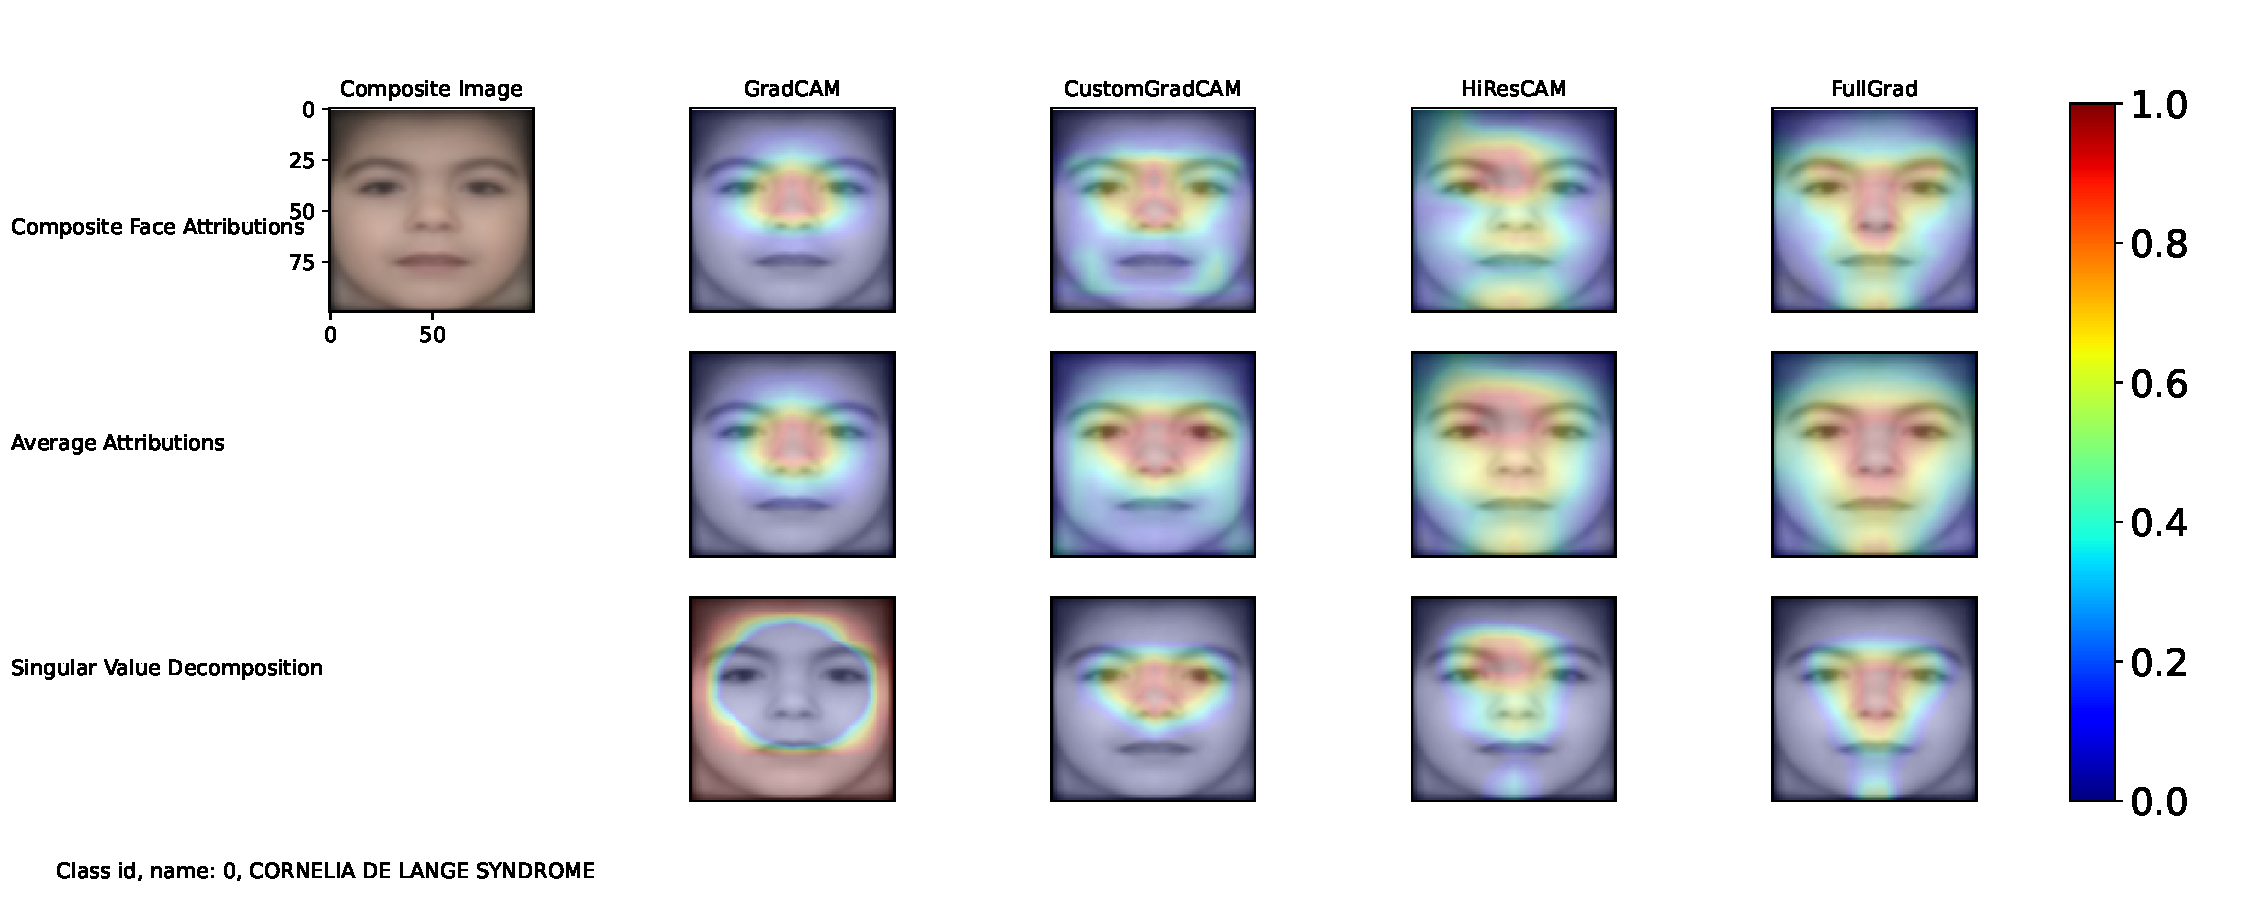
\includegraphics[scale=0.43]{chapter5/example_syndrome_wise_map.pdf}
		\caption{An example for syndrome-wise attribution maps}
		\label{fig_synd_maps}
	\end{figure}
	\end{enumerate}


    
    \subsection{Dataset Imbalance - Explanation Quality Analysis}
    
    
   \section{Evaluation Questionnaire}
\end{document}
